\documentclass[1p]{elsarticle_modified}
%\bibliographystyle{elsarticle-num}

%\usepackage[colorlinks]{hyperref}
%\usepackage{abbrmath_seonhwa} %\Abb, \Ascr, \Acal ,\Abf, \Afrak
\usepackage{amsfonts}
\usepackage{amssymb}
\usepackage{amsmath}
\usepackage{amsthm}
\usepackage{scalefnt}
\usepackage{amsbsy}
\usepackage{kotex}
\usepackage{caption}
\usepackage{subfig}
\usepackage{color}
\usepackage{graphicx}
\usepackage{xcolor} %% white, black, red, green, blue, cyan, magenta, yellow
\usepackage{float}
\usepackage{setspace}
\usepackage{hyperref}

\usepackage{tikz}
\usetikzlibrary{arrows}

\usepackage{multirow}
\usepackage{array} % fixed length table
\usepackage{hhline}

%%%%%%%%%%%%%%%%%%%%%
\makeatletter
\renewcommand*\env@matrix[1][\arraystretch]{%
	\edef\arraystretch{#1}%
	\hskip -\arraycolsep
	\let\@ifnextchar\new@ifnextchar
	\array{*\c@MaxMatrixCols c}}
\makeatother %https://tex.stackexchange.com/questions/14071/how-can-i-increase-the-line-spacing-in-a-matrix
%%%%%%%%%%%%%%%

\usepackage[normalem]{ulem}

\newcommand{\msout}[1]{\ifmmode\text{\sout{\ensuremath{#1}}}\else\sout{#1}\fi}
%SOURCE: \msout is \stkout macro in https://tex.stackexchange.com/questions/20609/strikeout-in-math-mode

\newcommand{\cancel}[1]{
	\ifmmode
	{\color{red}\msout{#1}}
	\else
	{\color{red}\sout{#1}}
	\fi
}

\newcommand{\add}[1]{
	{\color{blue}\uwave{#1}}
}

\newcommand{\replace}[2]{
	\ifmmode
	{\color{red}\msout{#1}}{\color{blue}\uwave{#2}}
	\else
	{\color{red}\sout{#1}}{\color{blue}\uwave{#2}}
	\fi
}

\newcommand{\Sol}{\mathcal{S}} %segment
\newcommand{\D}{D} %diagram
\newcommand{\A}{\mathcal{A}} %arc


%%%%%%%%%%%%%%%%%%%%%%%%%%%%%5 test

\def\sl{\operatorname{\textup{SL}}(2,\Cbb)}
\def\psl{\operatorname{\textup{PSL}}(2,\Cbb)}
\def\quan{\mkern 1mu \triangleright \mkern 1mu}

\theoremstyle{definition}
\newtheorem{thm}{Theorem}[section]
\newtheorem{prop}[thm]{Proposition}
\newtheorem{lem}[thm]{Lemma}
\newtheorem{ques}[thm]{Question}
\newtheorem{cor}[thm]{Corollary}
\newtheorem{defn}[thm]{Definition}
\newtheorem{exam}[thm]{Example}
\newtheorem{rmk}[thm]{Remark}
\newtheorem{alg}[thm]{Algorithm}

\newcommand{\I}{\sqrt{-1}}
\begin{document}

%\begin{frontmatter}
%
%\title{Boundary parabolic representations of knots up to 8 crossings}
%
%%% Group authors per affiliation:
%\author{Yunhi Cho} 
%\address{Department of Mathematics, University of Seoul, Seoul, Korea}
%\ead{yhcho@uos.ac.kr}
%
%
%\author{Seonhwa Kim} %\fnref{s_kim}}
%\address{Center for Geometry and Physics, Institute for Basic Science, Pohang, 37673, Korea}
%\ead{ryeona17@ibs.re.kr}
%
%\author{Hyuk Kim}
%\address{Department of Mathematical Sciences, Seoul National University, Seoul 08826, Korea}
%\ead{hyukkim@snu.ac.kr}
%
%\author{Seokbeom Yoon}
%\address{Department of Mathematical Sciences, Seoul National University, Seoul, 08826,  Korea}
%\ead{sbyoon15@snu.ac.kr}
%
%\begin{abstract}
%We find all boundary parabolic representation of knots up to 8 crossings.
%
%\end{abstract}
%\begin{keyword}
%    \MSC[2010] 57M25 
%\end{keyword}
%
%\end{frontmatter}

%\linenumbers
%\tableofcontents
%
\newcommand\colored[1]{\textcolor{white}{\rule[-0.35ex]{0.8em}{1.4ex}}\kern-0.8em\color{red} #1}%
%\newcommand\colored[1]{\textcolor{white}{ #1}\kern-2.17ex	\textcolor{white}{ #1}\kern-1.81ex	\textcolor{white}{ #1}\kern-2.15ex\color{red}#1	}

{\Large $\underline{12n_{0350}~(K12n_{0350})}$}

\setlength{\tabcolsep}{10pt}
\renewcommand{\arraystretch}{1.6}
\vspace{1cm}\begin{tabular}{m{100pt}>{\centering\arraybackslash}m{274pt}}
\multirow{5}{120pt}{
	\centering
	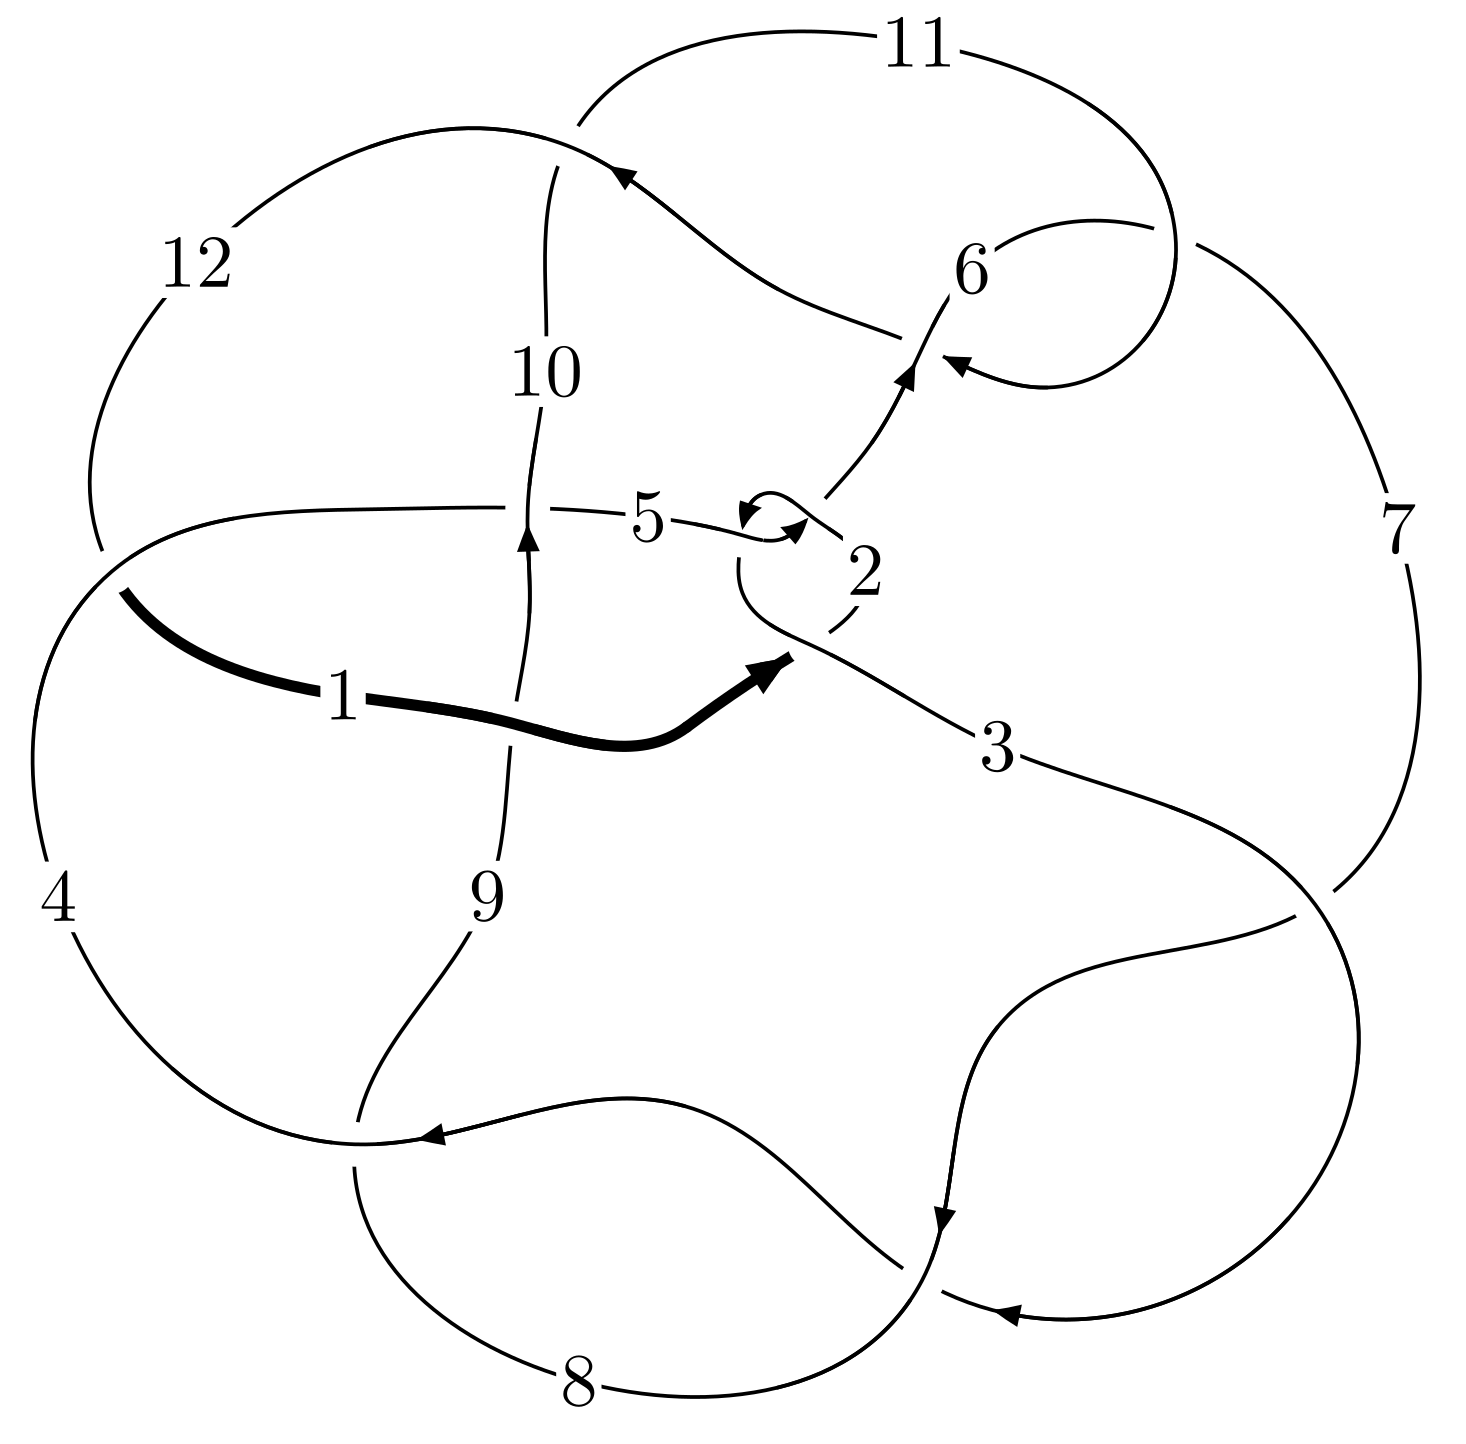
\includegraphics[width=112pt]{../../../GIT/diagram.site/Diagrams/png/2439_12n_0350.png}\\
\ \ \ A knot diagram\footnotemark}&
\allowdisplaybreaks
\textbf{Linearized knot diagam} \\
\cline{2-2}
 &
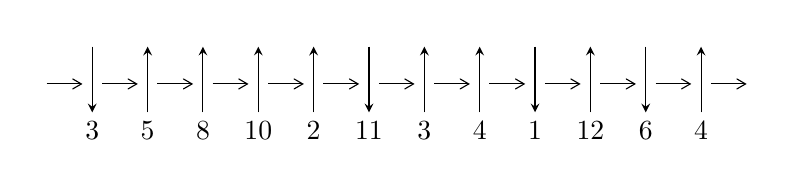
\begin{tikzpicture}[x=20pt, y=17pt]
	% nodes
	\node (C0) at (0, 0) {};
	\node (C1) at (1, 0) {};
	\node (C1U) at (1, +1) {};
	\node (C1D) at (1, -1) {3};

	\node (C2) at (2, 0) {};
	\node (C2U) at (2, +1) {};
	\node (C2D) at (2, -1) {5};

	\node (C3) at (3, 0) {};
	\node (C3U) at (3, +1) {};
	\node (C3D) at (3, -1) {8};

	\node (C4) at (4, 0) {};
	\node (C4U) at (4, +1) {};
	\node (C4D) at (4, -1) {10};

	\node (C5) at (5, 0) {};
	\node (C5U) at (5, +1) {};
	\node (C5D) at (5, -1) {2};

	\node (C6) at (6, 0) {};
	\node (C6U) at (6, +1) {};
	\node (C6D) at (6, -1) {11};

	\node (C7) at (7, 0) {};
	\node (C7U) at (7, +1) {};
	\node (C7D) at (7, -1) {3};

	\node (C8) at (8, 0) {};
	\node (C8U) at (8, +1) {};
	\node (C8D) at (8, -1) {4};

	\node (C9) at (9, 0) {};
	\node (C9U) at (9, +1) {};
	\node (C9D) at (9, -1) {1};

	\node (C10) at (10, 0) {};
	\node (C10U) at (10, +1) {};
	\node (C10D) at (10, -1) {12};

	\node (C11) at (11, 0) {};
	\node (C11U) at (11, +1) {};
	\node (C11D) at (11, -1) {6};

	\node (C12) at (12, 0) {};
	\node (C12U) at (12, +1) {};
	\node (C12D) at (12, -1) {4};
	\node (C13) at (13, 0) {};

	% arrows
	\draw[->,>={angle 60}]
	(C0) edge (C1) (C1) edge (C2) (C2) edge (C3) (C3) edge (C4) (C4) edge (C5) (C5) edge (C6) (C6) edge (C7) (C7) edge (C8) (C8) edge (C9) (C9) edge (C10) (C10) edge (C11) (C11) edge (C12) (C12) edge (C13) ;	\draw[->,>=stealth]
	(C1U) edge (C1D) (C2D) edge (C2U) (C3D) edge (C3U) (C4D) edge (C4U) (C5D) edge (C5U) (C6U) edge (C6D) (C7D) edge (C7U) (C8D) edge (C8U) (C9U) edge (C9D) (C10D) edge (C10U) (C11U) edge (C11D) (C12D) edge (C12U) ;
	\end{tikzpicture} \\
\hhline{~~} \\& 
\textbf{Solving Sequence} \\ \cline{2-2} 
 &
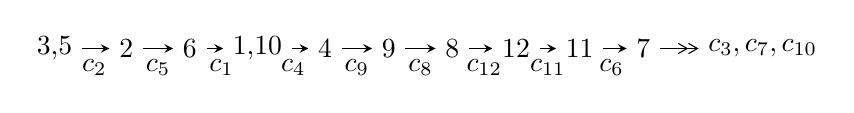
\begin{tikzpicture}[x=23pt, y=7pt]
	% node
	\node (A0) at (-1/8, 0) {3,5};
	\node (A1) at (1, 0) {2};
	\node (A2) at (2, 0) {6};
	\node (A3) at (49/16, 0) {1,10};
	\node (A4) at (33/8, 0) {4};
	\node (A5) at (41/8, 0) {9};
	\node (A6) at (49/8, 0) {8};
	\node (A7) at (57/8, 0) {12};
	\node (A8) at (65/8, 0) {11};
	\node (A9) at (73/8, 0) {7};
	\node (C1) at (1/2, -1) {$c_{2}$};
	\node (C2) at (3/2, -1) {$c_{5}$};
	\node (C3) at (5/2, -1) {$c_{1}$};
	\node (C4) at (29/8, -1) {$c_{4}$};
	\node (C5) at (37/8, -1) {$c_{9}$};
	\node (C6) at (45/8, -1) {$c_{8}$};
	\node (C7) at (53/8, -1) {$c_{12}$};
	\node (C8) at (61/8, -1) {$c_{11}$};
	\node (C9) at (69/8, -1) {$c_{6}$};
	\node (A10) at (11, 0) {$c_{3},c_{7},c_{10}$};

	% edge
	\draw[->,>=stealth]	
	(A0) edge (A1) (A1) edge (A2) (A2) edge (A3) (A3) edge (A4) (A4) edge (A5) (A5) edge (A6) (A6) edge (A7) (A7) edge (A8) (A8) edge (A9) ;
	\draw[->>,>={angle 60}]	
	(A9) edge (A10);
\end{tikzpicture} \\ 

\end{tabular} \\

\footnotetext{
The image of knot diagram is generated by the software ``\textbf{Draw programme}" developed by Andrew Bartholomew(\url{http://www.layer8.co.uk/maths/draw/index.htm\#Running-draw}), where we modified some parts for our purpose(\url{https://github.com/CATsTAILs/LinksPainter}).
}\phantom \\ \newline 
\centering \textbf{Ideals for irreducible components\footnotemark of $X_{\text{par}}$} 
 
\begin{align*}
I^u_{1}&=\langle 
-5.29491\times10^{120} u^{72}-5.67691\times10^{120} u^{71}+\cdots+2.16404\times10^{120} b+3.26172\times10^{122},\\
\phantom{I^u_{1}}&\phantom{= \langle  }-1.13483\times10^{122} u^{72}-2.62988\times10^{122} u^{71}+\cdots+3.09458\times10^{122} a-3.19287\times10^{124},\\
\phantom{I^u_{1}}&\phantom{= \langle  }u^{73}+u^{72}+\cdots-54 u+143\rangle \\
I^u_{2}&=\langle 
u^{21}+2 u^{20}+\cdots+b+2,\;-6 u^{21}-7 u^{20}+\cdots+a+7,\;u^{22}+2 u^{21}+\cdots+2 u+1\rangle \\
\\
\end{align*}
\raggedright * 2 irreducible components of $\dim_{\mathbb{C}}=0$, with total 95 representations.\\
\footnotetext{All coefficients of polynomials are rational numbers. But the coefficients are sometimes approximated in decimal forms when there is not enough margin.}
\newpage
\renewcommand{\arraystretch}{1}
\centering \section*{I. $I^u_{1}= \langle -5.29\times10^{120} u^{72}-5.68\times10^{120} u^{71}+\cdots+2.16\times10^{120} b+3.26\times10^{122},\;-1.13\times10^{122} u^{72}-2.63\times10^{122} u^{71}+\cdots+3.09\times10^{122} a-3.19\times10^{124},\;u^{73}+u^{72}+\cdots-54 u+143 \rangle$}
\flushleft \textbf{(i) Arc colorings}\\
\begin{tabular}{m{7pt} m{180pt} m{7pt} m{180pt} }
\flushright $a_{3}=$&$\begin{pmatrix}1\\0\end{pmatrix}$ \\
\flushright $a_{5}=$&$\begin{pmatrix}0\\u\end{pmatrix}$ \\
\flushright $a_{2}=$&$\begin{pmatrix}1\\u^2\end{pmatrix}$ \\
\flushright $a_{6}=$&$\begin{pmatrix}u\\u^3+u\end{pmatrix}$ \\
\flushright $a_{1}=$&$\begin{pmatrix}u^2+1\\u^2\end{pmatrix}$ \\
\flushright $a_{10}=$&$\begin{pmatrix}0.366715 u^{72}+0.849834 u^{71}+\cdots+93.7582 u+103.176\\2.44677 u^{72}+2.62329 u^{71}+\cdots+404.194 u-150.723\end{pmatrix}$ \\
\flushright $a_{4}=$&$\begin{pmatrix}-0.0790626 u^{72}-0.0854014 u^{71}+\cdots-11.2736 u-52.6707\\-0.461261 u^{72}+0.201291 u^{71}+\cdots-91.3359 u+152.246\end{pmatrix}$ \\
\flushright $a_{9}=$&$\begin{pmatrix}0.103382 u^{72}+0.154811 u^{71}+\cdots+68.5103 u+78.0723\\1.59212 u^{72}+1.90881 u^{71}+\cdots+288.755 u-68.9470\end{pmatrix}$ \\
\flushright $a_{8}=$&$\begin{pmatrix}-0.555398 u^{72}-1.64164 u^{71}+\cdots-56.7111 u-118.525\\0.235819 u^{72}+0.648309 u^{71}+\cdots+33.9399 u+52.7633\end{pmatrix}$ \\
\flushright $a_{12}=$&$\begin{pmatrix}-0.420761 u^{72}-0.753968 u^{71}+\cdots-88.3251 u+21.7494\\0.826324 u^{72}+0.838782 u^{71}+\cdots+168.780 u-9.30641\end{pmatrix}$ \\
\flushright $a_{11}=$&$\begin{pmatrix}-1.42862 u^{72}-1.96581 u^{71}+\cdots-265.577 u+38.5749\\0.600156 u^{72}+0.832821 u^{71}+\cdots+124.638 u+36.6878\end{pmatrix}$ \\
\flushright $a_{7}=$&$\begin{pmatrix}0.791216 u^{72}+2.28995 u^{71}+\cdots+90.6511 u+171.289\\-0.235819 u^{72}-0.648309 u^{71}+\cdots-33.9399 u-52.7633\end{pmatrix}$\\&\end{tabular}
\flushleft \textbf{(ii) Obstruction class $= -1$}\\~\\
\flushleft \textbf{(iii) Cusp Shapes $= -2.47879 u^{72}-1.95242 u^{71}+\cdots-309.552 u+200.317$}\\~\\
\newpage\renewcommand{\arraystretch}{1}
\flushleft \textbf{(iv) u-Polynomials at the component}\newline \\
\begin{tabular}{m{50pt}|m{274pt}}
Crossings & \hspace{64pt}u-Polynomials at each crossing \\
\hline $$\begin{aligned}c_{1}\end{aligned}$$&$\begin{aligned}
&u^{73}+43 u^{72}+\cdots-318262 u-20449
\end{aligned}$\\
\hline $$\begin{aligned}c_{2},c_{5}\end{aligned}$$&$\begin{aligned}
&u^{73}- u^{72}+\cdots-54 u-143
\end{aligned}$\\
\hline $$\begin{aligned}c_{3},c_{7},c_{8}\end{aligned}$$&$\begin{aligned}
&u^{73}+u^{72}+\cdots-18 u-1
\end{aligned}$\\
\hline $$\begin{aligned}c_{4}\end{aligned}$$&$\begin{aligned}
&u^{73}- u^{72}+\cdots-26 u-3
\end{aligned}$\\
\hline $$\begin{aligned}c_{6},c_{11}\end{aligned}$$&$\begin{aligned}
&u^{73}+u^{72}+\cdots+280 u-119
\end{aligned}$\\
\hline $$\begin{aligned}c_{9}\end{aligned}$$&$\begin{aligned}
&u^{73}-5 u^{72}+\cdots+22 u-1
\end{aligned}$\\
\hline $$\begin{aligned}c_{10}\end{aligned}$$&$\begin{aligned}
&u^{73}-25 u^{72}+\cdots-219576 u+14161
\end{aligned}$\\
\hline $$\begin{aligned}c_{12}\end{aligned}$$&$\begin{aligned}
&u^{73}+5 u^{72}+\cdots-14 u-1
\end{aligned}$\\
\hline
\end{tabular}\\~\\
\newpage\renewcommand{\arraystretch}{1}
\flushleft \textbf{(v) Riley Polynomials at the component}\newline \\
\begin{tabular}{m{50pt}|m{274pt}}
Crossings & \hspace{64pt}Riley Polynomials at each crossing \\
\hline $$\begin{aligned}c_{1}\end{aligned}$$&$\begin{aligned}
&y^{73}-13 y^{72}+\cdots+6813662274 y-418161601
\end{aligned}$\\
\hline $$\begin{aligned}c_{2},c_{5}\end{aligned}$$&$\begin{aligned}
&y^{73}+43 y^{72}+\cdots-318262 y-20449
\end{aligned}$\\
\hline $$\begin{aligned}c_{3},c_{7},c_{8}\end{aligned}$$&$\begin{aligned}
&y^{73}-19 y^{72}+\cdots+78 y-1
\end{aligned}$\\
\hline $$\begin{aligned}c_{4}\end{aligned}$$&$\begin{aligned}
&y^{73}-9 y^{72}+\cdots-140 y-9
\end{aligned}$\\
\hline $$\begin{aligned}c_{6},c_{11}\end{aligned}$$&$\begin{aligned}
&y^{73}+25 y^{72}+\cdots-219576 y-14161
\end{aligned}$\\
\hline $$\begin{aligned}c_{9}\end{aligned}$$&$\begin{aligned}
&y^{73}-71 y^{72}+\cdots+74 y-1
\end{aligned}$\\
\hline $$\begin{aligned}c_{10}\end{aligned}$$&$\begin{aligned}
&y^{73}+45 y^{72}+\cdots+7780282916 y-200533921
\end{aligned}$\\
\hline $$\begin{aligned}c_{12}\end{aligned}$$&$\begin{aligned}
&y^{73}+65 y^{72}+\cdots-124 y-1
\end{aligned}$\\
\hline
\end{tabular}\\~\\
\newpage\flushleft \textbf{(vi) Complex Volumes and Cusp Shapes}
$$\begin{array}{c|c|c}  
\text{Solutions to }I^u_{1}& \I (\text{vol} + \sqrt{-1}CS) & \text{Cusp shape}\\
 \hline 
\begin{aligned}
u &= \phantom{-}0.683574 + 0.741540 I \\
a &= \phantom{-}1.24911 - 0.93513 I \\
b &= \phantom{-}1.63585 + 0.41682 I\end{aligned}
 & \phantom{-}6.62976 + 3.45446 I & \phantom{-}12.33941 + 0. I\phantom{ +0.000000I} \\ \hline\begin{aligned}
u &= \phantom{-}0.683574 - 0.741540 I \\
a &= \phantom{-}1.24911 + 0.93513 I \\
b &= \phantom{-}1.63585 - 0.41682 I\end{aligned}
 & \phantom{-}6.62976 - 3.45446 I & \phantom{-}12.33941 + 0. I\phantom{ +0.000000I} \\ \hline\begin{aligned}
u &= -0.986818 + 0.037483 I \\
a &= \phantom{-}1.21894 - 0.96902 I \\
b &= \phantom{-}1.38473 - 0.39776 I\end{aligned}
 & -3.56549 - 3.25751 I & \phantom{-}4.00000 + 2.71745 I \\ \hline\begin{aligned}
u &= -0.986818 - 0.037483 I \\
a &= \phantom{-}1.21894 + 0.96902 I \\
b &= \phantom{-}1.38473 + 0.39776 I\end{aligned}
 & -3.56549 + 3.25751 I & \phantom{-}4.00000 - 2.71745 I \\ \hline\begin{aligned}
u &= -0.535723 + 0.826575 I \\
a &= \phantom{-}0.676203 + 0.430293 I \\
b &= \phantom{-}0.919141 - 0.126022 I\end{aligned}
 & \phantom{-}1.71374 - 1.35709 I & \phantom{-}6.26252 + 3.77195 I \\ \hline\begin{aligned}
u &= -0.535723 - 0.826575 I \\
a &= \phantom{-}0.676203 - 0.430293 I \\
b &= \phantom{-}0.919141 + 0.126022 I\end{aligned}
 & \phantom{-}1.71374 + 1.35709 I & \phantom{-}6.26252 - 3.77195 I \\ \hline\begin{aligned}
u &= \phantom{-}0.249076 + 0.988123 I \\
a &= \phantom{-}0.963692 - 0.195170 I \\
b &= \phantom{-}1.215860 - 0.565099 I\end{aligned}
 & -0.10064 + 5.52882 I & \phantom{-}4.00000 - 5.78158 I \\ \hline\begin{aligned}
u &= \phantom{-}0.249076 - 0.988123 I \\
a &= \phantom{-}0.963692 + 0.195170 I \\
b &= \phantom{-}1.215860 + 0.565099 I\end{aligned}
 & -0.10064 - 5.52882 I & \phantom{-}4.00000 + 5.78158 I \\ \hline\begin{aligned}
u &= -0.171086 + 1.013120 I \\
a &= -1.240710 + 0.320252 I \\
b &= \phantom{-}0.183330 + 0.223602 I\end{aligned}
 & -2.89227 - 2.61557 I & \phantom{-}4.00000 + 0. I\phantom{ +0.000000I} \\ \hline\begin{aligned}
u &= -0.171086 - 1.013120 I \\
a &= -1.240710 - 0.320252 I \\
b &= \phantom{-}0.183330 - 0.223602 I\end{aligned}
 & -2.89227 + 2.61557 I & \phantom{-}4.00000 + 0. I\phantom{ +0.000000I}\\
 \hline 
 \end{array}$$\newpage$$\begin{array}{c|c|c}  
\text{Solutions to }I^u_{1}& \I (\text{vol} + \sqrt{-1}CS) & \text{Cusp shape}\\
 \hline 
\begin{aligned}
u &= \phantom{-}0.948455 + 0.085623 I \\
a &= -0.82199 + 1.24099 I \\
b &= -1.332150 + 0.245893 I\end{aligned}
 & -4.43555 - 4.42989 I & \phantom{-}3.57907 + 2.45374 I \\ \hline\begin{aligned}
u &= \phantom{-}0.948455 - 0.085623 I \\
a &= -0.82199 - 1.24099 I \\
b &= -1.332150 - 0.245893 I\end{aligned}
 & -4.43555 + 4.42989 I & \phantom{-}3.57907 - 2.45374 I \\ \hline\begin{aligned}
u &= \phantom{-}0.230974 + 1.025990 I \\
a &= -0.529050 + 1.197620 I \\
b &= -2.28839 - 0.58000 I\end{aligned}
 & \phantom{-}2.79792 + 3.70869 I & \phantom{-0.000000 } 0 \\ \hline\begin{aligned}
u &= \phantom{-}0.230974 - 1.025990 I \\
a &= -0.529050 - 1.197620 I \\
b &= -2.28839 + 0.58000 I\end{aligned}
 & \phantom{-}2.79792 - 3.70869 I & \phantom{-0.000000 } 0 \\ \hline\begin{aligned}
u &= -0.753813 + 0.569849 I \\
a &= \phantom{-}0.007602 - 0.307173 I \\
b &= -0.253666 + 0.408703 I\end{aligned}
 & \phantom{-}2.13347 - 0.67945 I & \phantom{-}9.13563 + 0.70093 I \\ \hline\begin{aligned}
u &= -0.753813 - 0.569849 I \\
a &= \phantom{-}0.007602 + 0.307173 I \\
b &= -0.253666 - 0.408703 I\end{aligned}
 & \phantom{-}2.13347 + 0.67945 I & \phantom{-}9.13563 - 0.70093 I \\ \hline\begin{aligned}
u &= \phantom{-}0.228817 + 0.896549 I \\
a &= \phantom{-}0.273889 - 0.255136 I \\
b &= -1.97284 + 3.60878 I\end{aligned}
 & -4.04258 + 1.08271 I & \phantom{-}11.21709 - 7.54652 I \\ \hline\begin{aligned}
u &= \phantom{-}0.228817 - 0.896549 I \\
a &= \phantom{-}0.273889 + 0.255136 I \\
b &= -1.97284 - 3.60878 I\end{aligned}
 & -4.04258 - 1.08271 I & \phantom{-}11.21709 + 7.54652 I \\ \hline\begin{aligned}
u &= \phantom{-}0.451538 + 0.991597 I \\
a &= -0.661238 + 0.590058 I \\
b &= -1.04730 - 2.04932 I\end{aligned}
 & \phantom{-}1.15731 + 7.06397 I & \phantom{-0.000000 } 0 \\ \hline\begin{aligned}
u &= \phantom{-}0.451538 - 0.991597 I \\
a &= -0.661238 - 0.590058 I \\
b &= -1.04730 + 2.04932 I\end{aligned}
 & \phantom{-}1.15731 - 7.06397 I & \phantom{-0.000000 } 0\\
 \hline 
 \end{array}$$\newpage$$\begin{array}{c|c|c}  
\text{Solutions to }I^u_{1}& \I (\text{vol} + \sqrt{-1}CS) & \text{Cusp shape}\\
 \hline 
\begin{aligned}
u &= \phantom{-}1.072770 + 0.230198 I \\
a &= \phantom{-}0.85636 - 1.12907 I \\
b &= \phantom{-}1.38317 - 0.30370 I\end{aligned}
 & -3.02705 - 10.41650 I & \phantom{-0.000000 } 0 \\ \hline\begin{aligned}
u &= \phantom{-}1.072770 - 0.230198 I \\
a &= \phantom{-}0.85636 + 1.12907 I \\
b &= \phantom{-}1.38317 + 0.30370 I\end{aligned}
 & -3.02705 + 10.41650 I & \phantom{-0.000000 } 0 \\ \hline\begin{aligned}
u &= -0.612070 + 0.941386 I \\
a &= \phantom{-}0.565613 - 0.052080 I \\
b &= \phantom{-}1.02901 - 1.19145 I\end{aligned}
 & \phantom{-}1.08635 - 4.46104 I & \phantom{-0.000000 } 0 \\ \hline\begin{aligned}
u &= -0.612070 - 0.941386 I \\
a &= \phantom{-}0.565613 + 0.052080 I \\
b &= \phantom{-}1.02901 + 1.19145 I\end{aligned}
 & \phantom{-}1.08635 + 4.46104 I & \phantom{-0.000000 } 0 \\ \hline\begin{aligned}
u &= -0.836204 + 0.261291 I \\
a &= -1.33600 + 1.06634 I \\
b &= -1.35173 + 0.47656 I\end{aligned}
 & -4.10363 + 2.39606 I & \phantom{-}3.81600 - 2.35228 I \\ \hline\begin{aligned}
u &= -0.836204 - 0.261291 I \\
a &= -1.33600 - 1.06634 I \\
b &= -1.35173 - 0.47656 I\end{aligned}
 & -4.10363 - 2.39606 I & \phantom{-}3.81600 + 2.35228 I \\ \hline\begin{aligned}
u &= \phantom{-}0.291875 + 1.098960 I \\
a &= -0.464893 - 0.352121 I \\
b &= -1.62372 + 0.26942 I\end{aligned}
 & -3.74319 + 0.35423 I & \phantom{-0.000000 } 0 \\ \hline\begin{aligned}
u &= \phantom{-}0.291875 - 1.098960 I \\
a &= -0.464893 + 0.352121 I \\
b &= -1.62372 - 0.26942 I\end{aligned}
 & -3.74319 - 0.35423 I & \phantom{-0.000000 } 0 \\ \hline\begin{aligned}
u &= -0.814736 + 0.183028 I \\
a &= -0.960227 + 0.069320 I \\
b &= -0.330314 + 0.069183 I\end{aligned}
 & \phantom{-}3.36781 - 3.36881 I & \phantom{-}14.2825 + 3.4147 I \\ \hline\begin{aligned}
u &= -0.814736 - 0.183028 I \\
a &= -0.960227 - 0.069320 I \\
b &= -0.330314 - 0.069183 I\end{aligned}
 & \phantom{-}3.36781 + 3.36881 I & \phantom{-}14.2825 - 3.4147 I\\
 \hline 
 \end{array}$$\newpage$$\begin{array}{c|c|c}  
\text{Solutions to }I^u_{1}& \I (\text{vol} + \sqrt{-1}CS) & \text{Cusp shape}\\
 \hline 
\begin{aligned}
u &= -0.090816 + 0.822219 I \\
a &= -1.43478 + 0.31964 I \\
b &= -1.180510 + 0.536261 I\end{aligned}
 & -2.10787 + 1.28735 I & -0.94828 + 1.56152 I \\ \hline\begin{aligned}
u &= -0.090816 - 0.822219 I \\
a &= -1.43478 - 0.31964 I \\
b &= -1.180510 - 0.536261 I\end{aligned}
 & -2.10787 - 1.28735 I & -0.94828 - 1.56152 I \\ \hline\begin{aligned}
u &= \phantom{-}0.686083 + 0.978905 I \\
a &= -0.765292 + 1.051350 I \\
b &= -1.57564 - 0.25864 I\end{aligned}
 & \phantom{-}5.92171 + 1.85310 I & \phantom{-0.000000 } 0 \\ \hline\begin{aligned}
u &= \phantom{-}0.686083 - 0.978905 I \\
a &= -0.765292 - 1.051350 I \\
b &= -1.57564 + 0.25864 I\end{aligned}
 & \phantom{-}5.92171 - 1.85310 I & \phantom{-0.000000 } 0 \\ \hline\begin{aligned}
u &= \phantom{-}0.348220 + 0.717099 I \\
a &= \phantom{-}0.633784 + 1.212890 I \\
b &= \phantom{-}0.300550 - 0.658677 I\end{aligned}
 & \phantom{-}0.72632 - 2.98385 I & \phantom{-}2.65867 - 1.61148 I \\ \hline\begin{aligned}
u &= \phantom{-}0.348220 - 0.717099 I \\
a &= \phantom{-}0.633784 - 1.212890 I \\
b &= \phantom{-}0.300550 + 0.658677 I\end{aligned}
 & \phantom{-}0.72632 + 2.98385 I & \phantom{-}2.65867 + 1.61148 I \\ \hline\begin{aligned}
u &= \phantom{-}0.559248 + 0.542007 I \\
a &= \phantom{-}0.304713 - 0.769105 I \\
b &= \phantom{-}1.63410 - 0.28852 I\end{aligned}
 & \phantom{-}2.49213 - 2.99410 I & \phantom{-}10.23774 + 2.77464 I \\ \hline\begin{aligned}
u &= \phantom{-}0.559248 - 0.542007 I \\
a &= \phantom{-}0.304713 + 0.769105 I \\
b &= \phantom{-}1.63410 + 0.28852 I\end{aligned}
 & \phantom{-}2.49213 + 2.99410 I & \phantom{-}10.23774 - 2.77464 I \\ \hline\begin{aligned}
u &= \phantom{-}0.071021 + 0.771811 I \\
a &= \phantom{-}0.03076 - 1.73667 I \\
b &= \phantom{-}1.51208 + 1.30733 I\end{aligned}
 & \phantom{-}3.99461 - 2.09346 I & \phantom{-}4.40638 + 4.85697 I \\ \hline\begin{aligned}
u &= \phantom{-}0.071021 - 0.771811 I \\
a &= \phantom{-}0.03076 + 1.73667 I \\
b &= \phantom{-}1.51208 - 1.30733 I\end{aligned}
 & \phantom{-}3.99461 + 2.09346 I & \phantom{-}4.40638 - 4.85697 I\\
 \hline 
 \end{array}$$\newpage$$\begin{array}{c|c|c}  
\text{Solutions to }I^u_{1}& \I (\text{vol} + \sqrt{-1}CS) & \text{Cusp shape}\\
 \hline 
\begin{aligned}
u &= \phantom{-}0.550268 + 1.099350 I \\
a &= \phantom{-}0.621185 + 0.125940 I \\
b &= \phantom{-}2.03807 + 0.21438 I\end{aligned}
 & -1.98384 + 7.01266 I & \phantom{-0.000000 } 0 \\ \hline\begin{aligned}
u &= \phantom{-}0.550268 - 1.099350 I \\
a &= \phantom{-}0.621185 - 0.125940 I \\
b &= \phantom{-}2.03807 - 0.21438 I\end{aligned}
 & -1.98384 - 7.01266 I & \phantom{-0.000000 } 0 \\ \hline\begin{aligned}
u &= -0.851304 + 0.913176 I \\
a &= \phantom{-}0.798557 + 0.326350 I \\
b &= \phantom{-}1.068680 - 0.466872 I\end{aligned}
 & \phantom{-}2.18546 - 1.63429 I & \phantom{-0.000000 } 0 \\ \hline\begin{aligned}
u &= -0.851304 - 0.913176 I \\
a &= \phantom{-}0.798557 - 0.326350 I \\
b &= \phantom{-}1.068680 + 0.466872 I\end{aligned}
 & \phantom{-}2.18546 + 1.63429 I & \phantom{-0.000000 } 0 \\ \hline\begin{aligned}
u &= \phantom{-}0.656597 + 0.322411 I \\
a &= \phantom{-}0.009722 + 1.058680 I \\
b &= -0.153000 - 0.490916 I\end{aligned}
 & \phantom{-}0.19655 - 2.31294 I & \phantom{-}2.63030 + 3.93885 I \\ \hline\begin{aligned}
u &= \phantom{-}0.656597 - 0.322411 I \\
a &= \phantom{-}0.009722 - 1.058680 I \\
b &= -0.153000 + 0.490916 I\end{aligned}
 & \phantom{-}0.19655 + 2.31294 I & \phantom{-}2.63030 - 3.93885 I \\ \hline\begin{aligned}
u &= -0.910749 + 0.899481 I \\
a &= -0.681027 - 0.535163 I \\
b &= -0.994698 + 0.400858 I\end{aligned}
 & \phantom{-}2.24214 - 4.81846 I & \phantom{-0.000000 } 0 \\ \hline\begin{aligned}
u &= -0.910749 - 0.899481 I \\
a &= -0.681027 + 0.535163 I \\
b &= -0.994698 - 0.400858 I\end{aligned}
 & \phantom{-}2.24214 + 4.81846 I & \phantom{-0.000000 } 0 \\ \hline\begin{aligned}
u &= -0.347418 + 1.242890 I \\
a &= \phantom{-}0.897027 + 0.556994 I \\
b &= \phantom{-}2.36861 - 1.55566 I\end{aligned}
 & -8.62556 - 1.39524 I & \phantom{-0.000000 } 0 \\ \hline\begin{aligned}
u &= -0.347418 - 1.242890 I \\
a &= \phantom{-}0.897027 - 0.556994 I \\
b &= \phantom{-}2.36861 + 1.55566 I\end{aligned}
 & -8.62556 + 1.39524 I & \phantom{-0.000000 } 0\\
 \hline 
 \end{array}$$\newpage$$\begin{array}{c|c|c}  
\text{Solutions to }I^u_{1}& \I (\text{vol} + \sqrt{-1}CS) & \text{Cusp shape}\\
 \hline 
\begin{aligned}
u &= -0.327113 + 1.269160 I \\
a &= -0.447376 - 0.279699 I \\
b &= -0.885740 + 0.124459 I\end{aligned}
 & -3.06231 - 3.20525 I & \phantom{-0.000000 } 0 \\ \hline\begin{aligned}
u &= -0.327113 - 1.269160 I \\
a &= -0.447376 + 0.279699 I \\
b &= -0.885740 - 0.124459 I\end{aligned}
 & -3.06231 + 3.20525 I & \phantom{-0.000000 } 0 \\ \hline\begin{aligned}
u &= \phantom{-}0.307931 + 0.612364 I \\
a &= -1.29884 - 0.76584 I \\
b &= -0.944065 + 0.409129 I\end{aligned}
 & -2.61771 + 1.38695 I & \phantom{-}0.42548 - 4.72459 I \\ \hline\begin{aligned}
u &= \phantom{-}0.307931 - 0.612364 I \\
a &= -1.29884 + 0.76584 I \\
b &= -0.944065 - 0.409129 I\end{aligned}
 & -2.61771 - 1.38695 I & \phantom{-}0.42548 + 4.72459 I \\ \hline\begin{aligned}
u &= -0.585251 + 1.199500 I \\
a &= -0.552128 + 1.160950 I \\
b &= \phantom{-}0.338923 + 0.505424 I\end{aligned}
 & -6.87606 - 7.71394 I & \phantom{-0.000000 } 0 \\ \hline\begin{aligned}
u &= -0.585251 - 1.199500 I \\
a &= -0.552128 - 1.160950 I \\
b &= \phantom{-}0.338923 - 0.505424 I\end{aligned}
 & -6.87606 + 7.71394 I & \phantom{-0.000000 } 0 \\ \hline\begin{aligned}
u &= \phantom{-}0.526112 + 1.266110 I \\
a &= \phantom{-}0.986760 - 0.358538 I \\
b &= \phantom{-}2.22186 + 1.40051 I\end{aligned}
 & -8.04182 + 9.70758 I & \phantom{-0.000000 } 0 \\ \hline\begin{aligned}
u &= \phantom{-}0.526112 - 1.266110 I \\
a &= \phantom{-}0.986760 + 0.358538 I \\
b &= \phantom{-}2.22186 - 1.40051 I\end{aligned}
 & -8.04182 - 9.70758 I & \phantom{-0.000000 } 0 \\ \hline\begin{aligned}
u &= \phantom{-}0.417829 + 1.314000 I \\
a &= -0.640898 - 0.878070 I \\
b &= -0.077620 - 0.324517 I\end{aligned}
 & -8.85194 + 0.38418 I & \phantom{-0.000000 } 0 \\ \hline\begin{aligned}
u &= \phantom{-}0.417829 - 1.314000 I \\
a &= -0.640898 + 0.878070 I \\
b &= -0.077620 + 0.324517 I\end{aligned}
 & -8.85194 - 0.38418 I & \phantom{-0.000000 } 0\\
 \hline 
 \end{array}$$\newpage$$\begin{array}{c|c|c}  
\text{Solutions to }I^u_{1}& \I (\text{vol} + \sqrt{-1}CS) & \text{Cusp shape}\\
 \hline 
\begin{aligned}
u &= -0.154627 + 1.375210 I \\
a &= \phantom{-}0.222651 - 0.081323 I \\
b &= -0.502565 + 0.009919 I\end{aligned}
 & -4.25898 - 3.13951 I & \phantom{-0.000000 } 0 \\ \hline\begin{aligned}
u &= -0.154627 - 1.375210 I \\
a &= \phantom{-}0.222651 + 0.081323 I \\
b &= -0.502565 - 0.009919 I\end{aligned}
 & -4.25898 + 3.13951 I & \phantom{-0.000000 } 0 \\ \hline\begin{aligned}
u &= -0.472127 + 1.305790 I \\
a &= -0.970835 - 0.577427 I \\
b &= -2.14130 + 1.05133 I\end{aligned}
 & -7.75277 - 8.37018 I & \phantom{-0.000000 } 0 \\ \hline\begin{aligned}
u &= -0.472127 - 1.305790 I \\
a &= -0.970835 + 0.577427 I \\
b &= -2.14130 - 1.05133 I\end{aligned}
 & -7.75277 + 8.37018 I & \phantom{-0.000000 } 0 \\ \hline\begin{aligned}
u &= -0.485385 + 1.325740 I \\
a &= \phantom{-}0.538637 + 0.179909 I \\
b &= \phantom{-}0.864234 - 0.172690 I\end{aligned}
 & -1.09461 - 8.18682 I & \phantom{-0.000000 } 0 \\ \hline\begin{aligned}
u &= -0.485385 - 1.325740 I \\
a &= \phantom{-}0.538637 - 0.179909 I \\
b &= \phantom{-}0.864234 + 0.172690 I\end{aligned}
 & -1.09461 + 8.18682 I & \phantom{-0.000000 } 0 \\ \hline\begin{aligned}
u &= -0.50188 + 1.32442 I \\
a &= \phantom{-}0.375415 - 0.996617 I \\
b &= -0.455184 - 0.473111 I\end{aligned}
 & -7.57640 - 2.11236 I & \phantom{-0.000000 } 0 \\ \hline\begin{aligned}
u &= -0.50188 - 1.32442 I \\
a &= \phantom{-}0.375415 + 0.996617 I \\
b &= -0.455184 + 0.473111 I\end{aligned}
 & -7.57640 + 2.11236 I & \phantom{-0.000000 } 0 \\ \hline\begin{aligned}
u &= \phantom{-}0.62233 + 1.28194 I \\
a &= -1.069290 + 0.406801 I \\
b &= -2.07922 - 1.15092 I\end{aligned}
 & -6.3009 + 16.4753 I & \phantom{-0.000000 } 0 \\ \hline\begin{aligned}
u &= \phantom{-}0.62233 - 1.28194 I \\
a &= -1.069290 - 0.406801 I \\
b &= -2.07922 + 1.15092 I\end{aligned}
 & -6.3009 - 16.4753 I & \phantom{-0.000000 } 0\\
 \hline 
 \end{array}$$\newpage$$\begin{array}{c|c|c}  
\text{Solutions to }I^u_{1}& \I (\text{vol} + \sqrt{-1}CS) & \text{Cusp shape}\\
 \hline 
\begin{aligned}
u &= -0.548644\phantom{ +0.000000I} \\
a &= \phantom{-}0.938206\phantom{ +0.000000I} \\
b &= \phantom{-}0.336065\phantom{ +0.000000I}\end{aligned}
 & \phantom{-}0.951713\phantom{ +0.000000I} & \phantom{-}10.2780\phantom{ +0.000000I} \\ \hline\begin{aligned}
u &= \phantom{-}0.30872 + 1.43489 I \\
a &= \phantom{-}0.479050 + 0.788819 I \\
b &= -0.076582 + 0.370238 I\end{aligned}
 & -8.67982 - 5.51516 I & \phantom{-0.000000 } 0 \\ \hline\begin{aligned}
u &= \phantom{-}0.30872 - 1.43489 I \\
a &= \phantom{-}0.479050 - 0.788819 I \\
b &= -0.076582 - 0.370238 I\end{aligned}
 & -8.67982 + 5.51516 I & \phantom{-0.000000 } 0\\
 \hline 
 \end{array}$$\newpage\newpage\renewcommand{\arraystretch}{1}
\centering \section*{II. $I^u_{2}= \langle u^{21}+2 u^{20}+\cdots+b+2,\;-6 u^{21}-7 u^{20}+\cdots+a+7,\;u^{22}+2 u^{21}+\cdots+2 u+1 \rangle$}
\flushleft \textbf{(i) Arc colorings}\\
\begin{tabular}{m{7pt} m{180pt} m{7pt} m{180pt} }
\flushright $a_{3}=$&$\begin{pmatrix}1\\0\end{pmatrix}$ \\
\flushright $a_{5}=$&$\begin{pmatrix}0\\u\end{pmatrix}$ \\
\flushright $a_{2}=$&$\begin{pmatrix}1\\u^2\end{pmatrix}$ \\
\flushright $a_{6}=$&$\begin{pmatrix}u\\u^3+u\end{pmatrix}$ \\
\flushright $a_{1}=$&$\begin{pmatrix}u^2+1\\u^2\end{pmatrix}$ \\
\flushright $a_{10}=$&$\begin{pmatrix}6 u^{21}+7 u^{20}+\cdots+7 u-7\\- u^{21}-2 u^{20}+\cdots+5 u-2\end{pmatrix}$ \\
\flushright $a_{4}=$&$\begin{pmatrix}-6 u^{21}-13 u^{20}+\cdots-35 u-9\\- u^{20}-2 u^{19}+\cdots-3 u-2\end{pmatrix}$ \\
\flushright $a_{9}=$&$\begin{pmatrix}10 u^{21}+12 u^{20}+\cdots+13 u-11\\u^{21}+2 u^{20}+\cdots+9 u+1\end{pmatrix}$ \\
\flushright $a_{8}=$&$\begin{pmatrix}2 u^{21}-4 u^{20}+\cdots-18 u-19\\u^{21}+u^{20}+\cdots-5 u-6\end{pmatrix}$ \\
\flushright $a_{12}=$&$\begin{pmatrix}8 u^{21}+11 u^{20}+\cdots+13 u-11\\2 u^{21}+4 u^{20}+\cdots+10 u+1\end{pmatrix}$ \\
\flushright $a_{11}=$&$\begin{pmatrix}8 u^{21}+10 u^{20}+\cdots+10 u-15\\3 u^{21}+5 u^{20}+\cdots+9 u-2\end{pmatrix}$ \\
\flushright $a_{7}=$&$\begin{pmatrix}u^{21}-5 u^{20}+\cdots-13 u-13\\u^{21}+u^{20}+\cdots-5 u-6\end{pmatrix}$\\&\end{tabular}
\flushleft \textbf{(ii) Obstruction class $= 1$}\\~\\
\flushleft \textbf{(iii) Cusp Shapes $= -6 u^{21}-9 u^{20}-34 u^{19}-38 u^{18}-100 u^{17}-95 u^{16}-208 u^{15}-158 u^{14}-307 u^{13}-182 u^{12}-348 u^{11}-137 u^{10}-288 u^9-36 u^8-183 u^7+43 u^6-64 u^5+69 u^4-21 u^3+45 u^2-4 u+20$}\\~\\
\newpage\renewcommand{\arraystretch}{1}
\flushleft \textbf{(iv) u-Polynomials at the component}\newline \\
\begin{tabular}{m{50pt}|m{274pt}}
Crossings & \hspace{64pt}u-Polynomials at each crossing \\
\hline $$\begin{aligned}c_{1}\end{aligned}$$&$\begin{aligned}
&u^{22}-12 u^{21}+\cdots-16 u+1
\end{aligned}$\\
\hline $$\begin{aligned}c_{2}\end{aligned}$$&$\begin{aligned}
&u^{22}+2 u^{21}+\cdots+2 u+1
\end{aligned}$\\
\hline $$\begin{aligned}c_{3}\end{aligned}$$&$\begin{aligned}
&u^{22}-9 u^{20}+\cdots-8 u^2+1
\end{aligned}$\\
\hline $$\begin{aligned}c_{4}\end{aligned}$$&$\begin{aligned}
&u^{22}-6 u^{20}+\cdots+5 u^2+1
\end{aligned}$\\
\hline $$\begin{aligned}c_{5}\end{aligned}$$&$\begin{aligned}
&u^{22}-2 u^{21}+\cdots-2 u+1
\end{aligned}$\\
\hline $$\begin{aligned}c_{6}\end{aligned}$$&$\begin{aligned}
&u^{22}-2 u^{21}+\cdots-2 u+1
\end{aligned}$\\
\hline $$\begin{aligned}c_{7},c_{8}\end{aligned}$$&$\begin{aligned}
&u^{22}-9 u^{20}+\cdots-8 u^2+1
\end{aligned}$\\
\hline $$\begin{aligned}c_{9}\end{aligned}$$&$\begin{aligned}
&u^{22}-2 u^{21}+\cdots+4 u^2+1
\end{aligned}$\\
\hline $$\begin{aligned}c_{10}\end{aligned}$$&$\begin{aligned}
&u^{22}+10 u^{21}+\cdots+18 u+1
\end{aligned}$\\
\hline $$\begin{aligned}c_{11}\end{aligned}$$&$\begin{aligned}
&u^{22}+2 u^{21}+\cdots+2 u+1
\end{aligned}$\\
\hline $$\begin{aligned}c_{12}\end{aligned}$$&$\begin{aligned}
&u^{22}+9 u^{20}+\cdots+7 u^2+1
\end{aligned}$\\
\hline
\end{tabular}\\~\\
\newpage\renewcommand{\arraystretch}{1}
\flushleft \textbf{(v) Riley Polynomials at the component}\newline \\
\begin{tabular}{m{50pt}|m{274pt}}
Crossings & \hspace{64pt}Riley Polynomials at each crossing \\
\hline $$\begin{aligned}c_{1}\end{aligned}$$&$\begin{aligned}
&y^{22}+8 y^{21}+\cdots-8 y+1
\end{aligned}$\\
\hline $$\begin{aligned}c_{2},c_{5}\end{aligned}$$&$\begin{aligned}
&y^{22}+12 y^{21}+\cdots+16 y+1
\end{aligned}$\\
\hline $$\begin{aligned}c_{3},c_{7},c_{8}\end{aligned}$$&$\begin{aligned}
&y^{22}-18 y^{21}+\cdots-16 y+1
\end{aligned}$\\
\hline $$\begin{aligned}c_{4}\end{aligned}$$&$\begin{aligned}
&y^{22}-12 y^{21}+\cdots+10 y+1
\end{aligned}$\\
\hline $$\begin{aligned}c_{6},c_{11}\end{aligned}$$&$\begin{aligned}
&y^{22}+10 y^{21}+\cdots+18 y+1
\end{aligned}$\\
\hline $$\begin{aligned}c_{9}\end{aligned}$$&$\begin{aligned}
&y^{22}-14 y^{21}+\cdots+8 y+1
\end{aligned}$\\
\hline $$\begin{aligned}c_{10}\end{aligned}$$&$\begin{aligned}
&y^{22}+2 y^{21}+\cdots-18 y+1
\end{aligned}$\\
\hline $$\begin{aligned}c_{12}\end{aligned}$$&$\begin{aligned}
&y^{22}+18 y^{21}+\cdots+14 y+1
\end{aligned}$\\
\hline
\end{tabular}\\~\\
\newpage\flushleft \textbf{(vi) Complex Volumes and Cusp Shapes}
$$\begin{array}{c|c|c}  
\text{Solutions to }I^u_{2}& \I (\text{vol} + \sqrt{-1}CS) & \text{Cusp shape}\\
 \hline 
\begin{aligned}
u &= -0.241973 + 0.958544 I \\
a &= -0.490866 + 0.123430 I \\
b &= -2.10277 - 2.55701 I\end{aligned}
 & -4.38986 - 0.97753 I & -11.44106 + 0.80561 I \\ \hline\begin{aligned}
u &= -0.241973 - 0.958544 I \\
a &= -0.490866 - 0.123430 I \\
b &= -2.10277 + 2.55701 I\end{aligned}
 & -4.38986 + 0.97753 I & -11.44106 - 0.80561 I \\ \hline\begin{aligned}
u &= \phantom{-}0.680342 + 0.808019 I \\
a &= -1.11141 + 1.19166 I \\
b &= -1.44518 - 0.36748 I\end{aligned}
 & \phantom{-}6.14692 + 4.23019 I & \phantom{-}6.87486 - 8.22378 I \\ \hline\begin{aligned}
u &= \phantom{-}0.680342 - 0.808019 I \\
a &= -1.11141 - 1.19166 I \\
b &= -1.44518 + 0.36748 I\end{aligned}
 & \phantom{-}6.14692 - 4.23019 I & \phantom{-}6.87486 + 8.22378 I \\ \hline\begin{aligned}
u &= \phantom{-}0.381053 + 0.993854 I \\
a &= \phantom{-}0.485823 - 0.931803 I \\
b &= \phantom{-}2.51178 + 0.40690 I\end{aligned}
 & \phantom{-}3.50530 + 4.41296 I & \phantom{-}8.17984 - 7.57278 I \\ \hline\begin{aligned}
u &= \phantom{-}0.381053 - 0.993854 I \\
a &= \phantom{-}0.485823 + 0.931803 I \\
b &= \phantom{-}2.51178 - 0.40690 I\end{aligned}
 & \phantom{-}3.50530 - 4.41296 I & \phantom{-}8.17984 + 7.57278 I \\ \hline\begin{aligned}
u &= -0.864576 + 0.756693 I \\
a &= -0.705540 - 0.375538 I \\
b &= -0.712469 + 0.591982 I\end{aligned}
 & \phantom{-}3.13466 - 4.55728 I & \phantom{-}13.4598 + 7.0179 I \\ \hline\begin{aligned}
u &= -0.864576 - 0.756693 I \\
a &= -0.705540 + 0.375538 I \\
b &= -0.712469 - 0.591982 I\end{aligned}
 & \phantom{-}3.13466 + 4.55728 I & \phantom{-}13.4598 - 7.0179 I \\ \hline\begin{aligned}
u &= \phantom{-}0.344344 + 0.775789 I \\
a &= -0.23930 + 1.47914 I \\
b &= -1.60383 - 1.37208 I\end{aligned}
 & \phantom{-}4.32626 - 1.33597 I & \phantom{-}9.03146 - 2.86152 I \\ \hline\begin{aligned}
u &= \phantom{-}0.344344 - 0.775789 I \\
a &= -0.23930 - 1.47914 I \\
b &= -1.60383 + 1.37208 I\end{aligned}
 & \phantom{-}4.32626 + 1.33597 I & \phantom{-}9.03146 + 2.86152 I\\
 \hline 
 \end{array}$$\newpage$$\begin{array}{c|c|c}  
\text{Solutions to }I^u_{2}& \I (\text{vol} + \sqrt{-1}CS) & \text{Cusp shape}\\
 \hline 
\begin{aligned}
u &= \phantom{-}0.683857 + 0.953567 I \\
a &= \phantom{-}0.986932 - 0.976839 I \\
b &= \phantom{-}1.58711 + 0.21263 I\end{aligned}
 & \phantom{-}5.68936 + 1.04482 I & \phantom{-}6.35421 + 3.19394 I \\ \hline\begin{aligned}
u &= \phantom{-}0.683857 - 0.953567 I \\
a &= \phantom{-}0.986932 + 0.976839 I \\
b &= \phantom{-}1.58711 - 0.21263 I\end{aligned}
 & \phantom{-}5.68936 - 1.04482 I & \phantom{-}6.35421 - 3.19394 I \\ \hline\begin{aligned}
u &= -0.483198 + 1.148360 I \\
a &= \phantom{-}0.511255 - 0.042735 I \\
b &= \phantom{-}1.178750 + 0.403621 I\end{aligned}
 & -1.14942 - 7.14765 I & \phantom{-}5.07018 + 7.28569 I \\ \hline\begin{aligned}
u &= -0.483198 - 1.148360 I \\
a &= \phantom{-}0.511255 + 0.042735 I \\
b &= \phantom{-}1.178750 - 0.403621 I\end{aligned}
 & -1.14942 + 7.14765 I & \phantom{-}5.07018 - 7.28569 I \\ \hline\begin{aligned}
u &= -0.887565 + 0.930577 I \\
a &= \phantom{-}0.669634 + 0.226011 I \\
b &= \phantom{-}0.920717 - 0.461715 I\end{aligned}
 & \phantom{-}2.63405 - 1.92174 I & \phantom{-}16.1641 + 7.0514 I \\ \hline\begin{aligned}
u &= -0.887565 - 0.930577 I \\
a &= \phantom{-}0.669634 - 0.226011 I \\
b &= \phantom{-}0.920717 + 0.461715 I\end{aligned}
 & \phantom{-}2.63405 + 1.92174 I & \phantom{-}16.1641 - 7.0514 I \\ \hline\begin{aligned}
u &= -0.182700 + 1.302970 I \\
a &= -0.532890 + 0.197172 I \\
b &= \phantom{-}0.140687 + 0.127074 I\end{aligned}
 & -4.66681 - 2.93382 I & -4.96536 - 0.66259 I \\ \hline\begin{aligned}
u &= -0.182700 - 1.302970 I \\
a &= -0.532890 - 0.197172 I \\
b &= \phantom{-}0.140687 - 0.127074 I\end{aligned}
 & -4.66681 + 2.93382 I & -4.96536 + 0.66259 I \\ \hline\begin{aligned}
u &= -0.321038 + 0.588930 I \\
a &= \phantom{-}0.76251 - 1.19934 I \\
b &= \phantom{-}0.970661 + 0.503731 I\end{aligned}
 & \phantom{-}1.05601 + 3.62165 I & \phantom{-}7.15284 - 7.64302 I \\ \hline\begin{aligned}
u &= -0.321038 - 0.588930 I \\
a &= \phantom{-}0.76251 + 1.19934 I \\
b &= \phantom{-}0.970661 - 0.503731 I\end{aligned}
 & \phantom{-}1.05601 - 3.62165 I & \phantom{-}7.15284 + 7.64302 I\\
 \hline 
 \end{array}$$\newpage$$\begin{array}{c|c|c}  
\text{Solutions to }I^u_{2}& \I (\text{vol} + \sqrt{-1}CS) & \text{Cusp shape}\\
 \hline 
\begin{aligned}
u &= -0.108546 + 0.545335 I \\
a &= -2.33615 + 0.39651 I \\
b &= -0.945452 + 0.497914 I\end{aligned}
 & -1.48208 + 1.54693 I & \phantom{-}10.61918 - 2.30760 I \\ \hline\begin{aligned}
u &= -0.108546 - 0.545335 I \\
a &= -2.33615 - 0.39651 I \\
b &= -0.945452 - 0.497914 I\end{aligned}
 & -1.48208 - 1.54693 I & \phantom{-}10.61918 + 2.30760 I\\
 \hline 
 \end{array}$$\newpage
\newpage\renewcommand{\arraystretch}{1}
\centering \section*{ III. u-Polynomials}
\begin{tabular}{m{50pt}|m{274pt}}
Crossings & \hspace{64pt}u-Polynomials at each crossing \\
\hline $$\begin{aligned}c_{1}\end{aligned}$$&$\begin{aligned}
&(u^{22}-12 u^{21}+\cdots-16 u+1)(u^{73}+43 u^{72}+\cdots-318262 u-20449)
\end{aligned}$\\
\hline $$\begin{aligned}c_{2}\end{aligned}$$&$\begin{aligned}
&(u^{22}+2 u^{21}+\cdots+2 u+1)(u^{73}- u^{72}+\cdots-54 u-143)
\end{aligned}$\\
\hline $$\begin{aligned}c_{3}\end{aligned}$$&$\begin{aligned}
&(u^{22}-9 u^{20}+\cdots-8 u^2+1)(u^{73}+u^{72}+\cdots-18 u-1)
\end{aligned}$\\
\hline $$\begin{aligned}c_{4}\end{aligned}$$&$\begin{aligned}
&(u^{22}-6 u^{20}+\cdots+5 u^2+1)(u^{73}- u^{72}+\cdots-26 u-3)
\end{aligned}$\\
\hline $$\begin{aligned}c_{5}\end{aligned}$$&$\begin{aligned}
&(u^{22}-2 u^{21}+\cdots-2 u+1)(u^{73}- u^{72}+\cdots-54 u-143)
\end{aligned}$\\
\hline $$\begin{aligned}c_{6}\end{aligned}$$&$\begin{aligned}
&(u^{22}-2 u^{21}+\cdots-2 u+1)(u^{73}+u^{72}+\cdots+280 u-119)
\end{aligned}$\\
\hline $$\begin{aligned}c_{7},c_{8}\end{aligned}$$&$\begin{aligned}
&(u^{22}-9 u^{20}+\cdots-8 u^2+1)(u^{73}+u^{72}+\cdots-18 u-1)
\end{aligned}$\\
\hline $$\begin{aligned}c_{9}\end{aligned}$$&$\begin{aligned}
&(u^{22}-2 u^{21}+\cdots+4 u^2+1)(u^{73}-5 u^{72}+\cdots+22 u-1)
\end{aligned}$\\
\hline $$\begin{aligned}c_{10}\end{aligned}$$&$\begin{aligned}
&(u^{22}+10 u^{21}+\cdots+18 u+1)(u^{73}-25 u^{72}+\cdots-219576 u+14161)
\end{aligned}$\\
\hline $$\begin{aligned}c_{11}\end{aligned}$$&$\begin{aligned}
&(u^{22}+2 u^{21}+\cdots+2 u+1)(u^{73}+u^{72}+\cdots+280 u-119)
\end{aligned}$\\
\hline $$\begin{aligned}c_{12}\end{aligned}$$&$\begin{aligned}
&(u^{22}+9 u^{20}+\cdots+7 u^2+1)(u^{73}+5 u^{72}+\cdots-14 u-1)
\end{aligned}$\\
\hline
\end{tabular}\newpage\renewcommand{\arraystretch}{1}
\centering \section*{ IV. Riley Polynomials}
\begin{tabular}{m{50pt}|m{274pt}}
Crossings & \hspace{64pt}Riley Polynomials at each crossing \\
\hline $$\begin{aligned}c_{1}\end{aligned}$$&$\begin{aligned}
&(y^{22}+8 y^{21}+\cdots-8 y+1)\\
&\cdot(y^{73}-13 y^{72}+\cdots+6813662274 y-418161601)
\end{aligned}$\\
\hline $$\begin{aligned}c_{2},c_{5}\end{aligned}$$&$\begin{aligned}
&(y^{22}+12 y^{21}+\cdots+16 y+1)(y^{73}+43 y^{72}+\cdots-318262 y-20449)
\end{aligned}$\\
\hline $$\begin{aligned}c_{3},c_{7},c_{8}\end{aligned}$$&$\begin{aligned}
&(y^{22}-18 y^{21}+\cdots-16 y+1)(y^{73}-19 y^{72}+\cdots+78 y-1)
\end{aligned}$\\
\hline $$\begin{aligned}c_{4}\end{aligned}$$&$\begin{aligned}
&(y^{22}-12 y^{21}+\cdots+10 y+1)(y^{73}-9 y^{72}+\cdots-140 y-9)
\end{aligned}$\\
\hline $$\begin{aligned}c_{6},c_{11}\end{aligned}$$&$\begin{aligned}
&(y^{22}+10 y^{21}+\cdots+18 y+1)(y^{73}+25 y^{72}+\cdots-219576 y-14161)
\end{aligned}$\\
\hline $$\begin{aligned}c_{9}\end{aligned}$$&$\begin{aligned}
&(y^{22}-14 y^{21}+\cdots+8 y+1)(y^{73}-71 y^{72}+\cdots+74 y-1)
\end{aligned}$\\
\hline $$\begin{aligned}c_{10}\end{aligned}$$&$\begin{aligned}
&(y^{22}+2 y^{21}+\cdots-18 y+1)\\
&\cdot(y^{73}+45 y^{72}+\cdots+7780282916 y-200533921)
\end{aligned}$\\
\hline $$\begin{aligned}c_{12}\end{aligned}$$&$\begin{aligned}
&(y^{22}+18 y^{21}+\cdots+14 y+1)(y^{73}+65 y^{72}+\cdots-124 y-1)
\end{aligned}$\\
\hline
\end{tabular}
\vskip 2pc
\end{document}